\documentclass[../DCM2_Verslag.tex]{subfiles}
\begin{document}


\section{Resultaten}
\subsection{Baseline}
	\begin{tabular}{||l|c|r|p{6cm}||}
   	 Testsoort & Bandbreedte (gemiddelde na 3 testen)\\
   	 \hline \hline    
   	 UDP RX &  \\
   	 UDP TX &  \\
   	 TCP TX & \\
   	 TCP RX &  \\
   	 \hline
	\end{tabular}

\subsection{Window sizes}

\subsubsection{Window sizes test met ESP32 als server}
	\begin{tabular}{||l|c|r|p{6cm}||}
   	 Package size(bytes) & Bandbreedte (gemiddelde na 3 testen) & Latency\\
   	 \hline \hline    
   	 4 KB &  & \\
   	 8 KB &  & \\
   	 16 KB & & \\
   	 32 KB &  & \\
   	 64 KB & & \\
   	 128 KB & & \\
   	 256 KB & & \\
   	 400 KB & &\\
   	 \hline
	\end{tabular}
	
	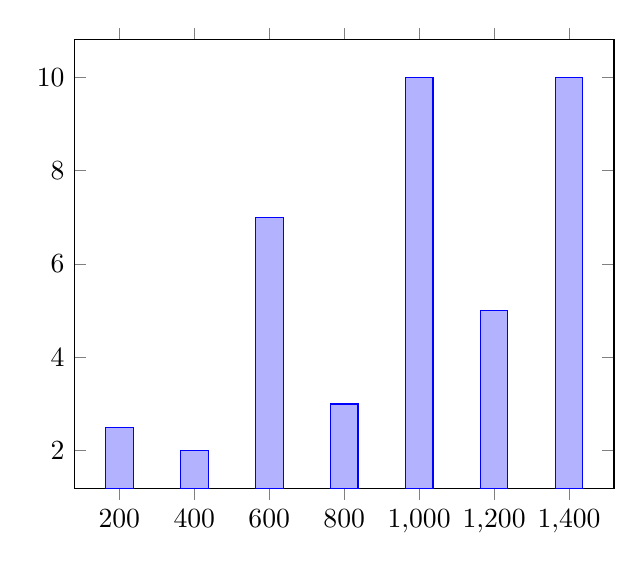
\begin{tikzpicture}
	\begin{axis} [ybar]
	\addplot coordinates {
    (200,2.5) 
    (400,2)
	(600,7)
    (800,3)
	(1000, 10)
	(1200,5)
	(1400,10)
	};
\end{axis}
\end{tikzpicture}

\subsubsection{Window sizes test met ESP32 als client}
	\begin{tabular}{||l|c|r|p{6cm}||}
   	 Package size(bytes) & Bandbreedte (gemiddelde na 3 testen) & Latency\\
   	 \hline \hline    
   	 4 KB &  & \\
   	 8 KB &  & \\
   	 16 KB & & \\
   	 32 KB &  & \\
   	 64 KB & & \\
   	 128 KB & & \\
   	 256 KB & & \\
   	 400 KB & &\\
   	 \hline
	\end{tabular}
	
	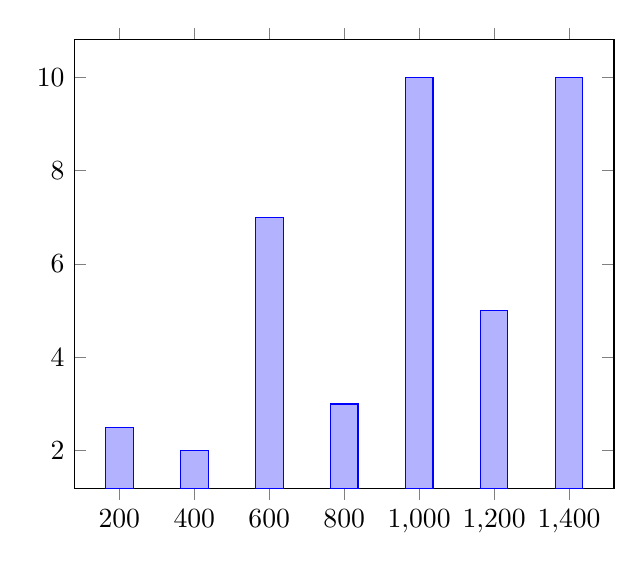
\begin{tikzpicture}
	\begin{axis} [ybar]
	\addplot coordinates {
    (200,2.5) 
    (400,2)
	(600,7)
    (800,3)
	(1000, 10)
	(1200,5)
	(1400,10)
	};
\end{axis}
\end{tikzpicture}

\subsection{Package sizes}


\subsubsection{Package sizes test met ESP32 als server}
	\begin{tabular}{||l|c|r|p{6cm}||}
   	 Package size(bytes) & Bandbreedte (gemiddelde na 3 testen)\\
   	 \hline \hline    
   	 200 bytes (160 bytes MSS) &  \\
   	 400 bytes (360 bytes MSS) &  \\
   	 600 bytes (560 bytes MSS) &  \\
   	 800 bytes (760 bytes MSS) &  \\
   	 1000 bytes (960 bytes MSS) & \\
   	 1200 bytes (1160 bytes MSS) &  \\
   	 1400 bytes (1360 bytes MSS) & \\
   	 \hline
	\end{tabular}
	
	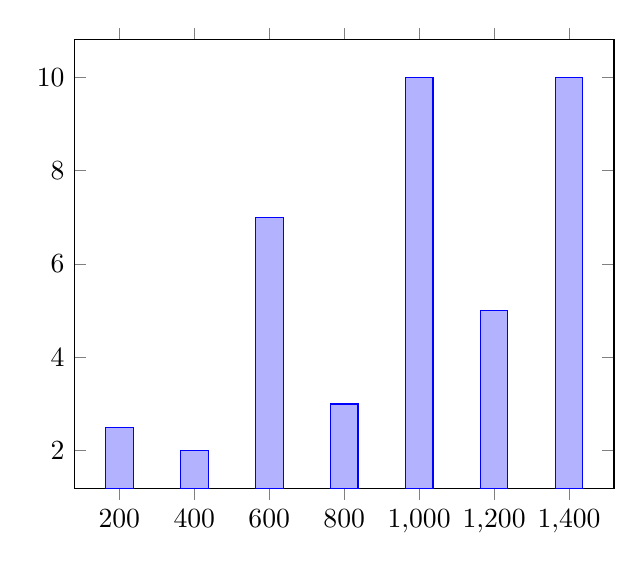
\begin{tikzpicture}
	\begin{axis} [ybar]
	\addplot coordinates {
    (200,2.5) 
    (400,2)
	(600,7)
    (800,3)
	(1000, 10)
	(1200,5)
	(1400,10)
	};
\end{axis}
\end{tikzpicture}

\subsubsection{Package sizes test met ESP32 als client}
	\begin{tabular}{||l|c|r|p{6cm}||}
   	 Package size(bytes) & Bandbreedte (gemiddelde na 3 testen)\\
   	 \hline \hline    
   	 200 bytes (160 bytes MSS) &  \\
   	 400 bytes (360 bytes MSS) &  \\
   	 600 bytes (560 bytes MSS) &  \\
   	 800 bytes (760 bytes MSS) &  \\
   	 1000 bytes (960 bytes MSS) & \\
   	 1200 bytes (1160 bytes MSS) &  \\
   	 1400 bytes (1360 bytes MSS) & \\
   	 \hline
	\end{tabular}
	
	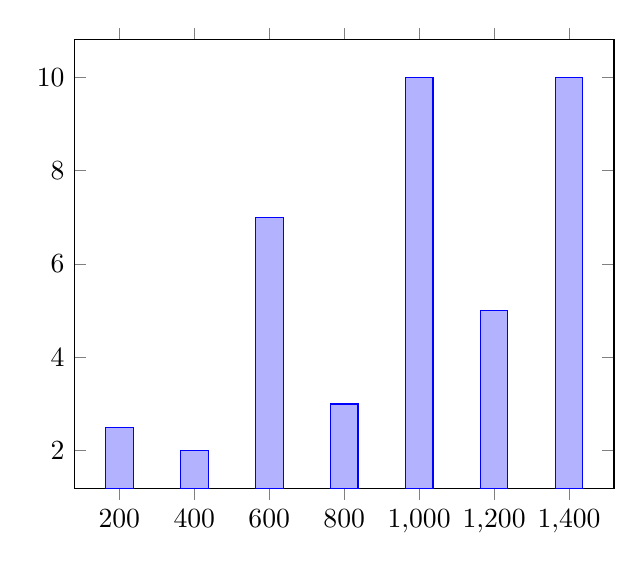
\begin{tikzpicture}
	\begin{axis} [ybar]
	\addplot coordinates {
    (200,2.5) 
    (400,2)
	(600,7)
    (800,3)
	(1000, 10)
	(1200,5)
	(1400,10)
	};
\end{axis}
\end{tikzpicture}



\end{document}
